% !TeX spellcheck = en_US

\chapter{Results}
\label{chap:results}
For this project we have chosen to use \CC17 and to implement a multi-threaded program to achieve a better execution time upon the computational process using OpenMP, an open standard for parallelism for C, C++ and Fortran programs. The whole execution has been run on a cluster of $10$ \texttt{Intel(R) Xeon(R) CPU E5430 @ 2.66GHz - 16GB RAM}. With this computational power, we have been able to perform multiple experiments by varying the $K$-fold value in the cross-validation: $2$, $3$, $5$, $10$, $20$, $50$, $150$, $300$, $750$ during a period of seven days of computation. With this cluster we have been able to calculate the loss function for any single iteration.\\
The program has been written to print all the results in a \texttt{.json} file to achieve an easier data analysis through Python. In all of the experiments, both AdaBoost and Bagging have been trained over the whole data-set with the same hyper-parameter $T$ for each iteration.\\
\begin{figure}
	\centering
	\subfloat[K = 2]{
		\label{ref_k2}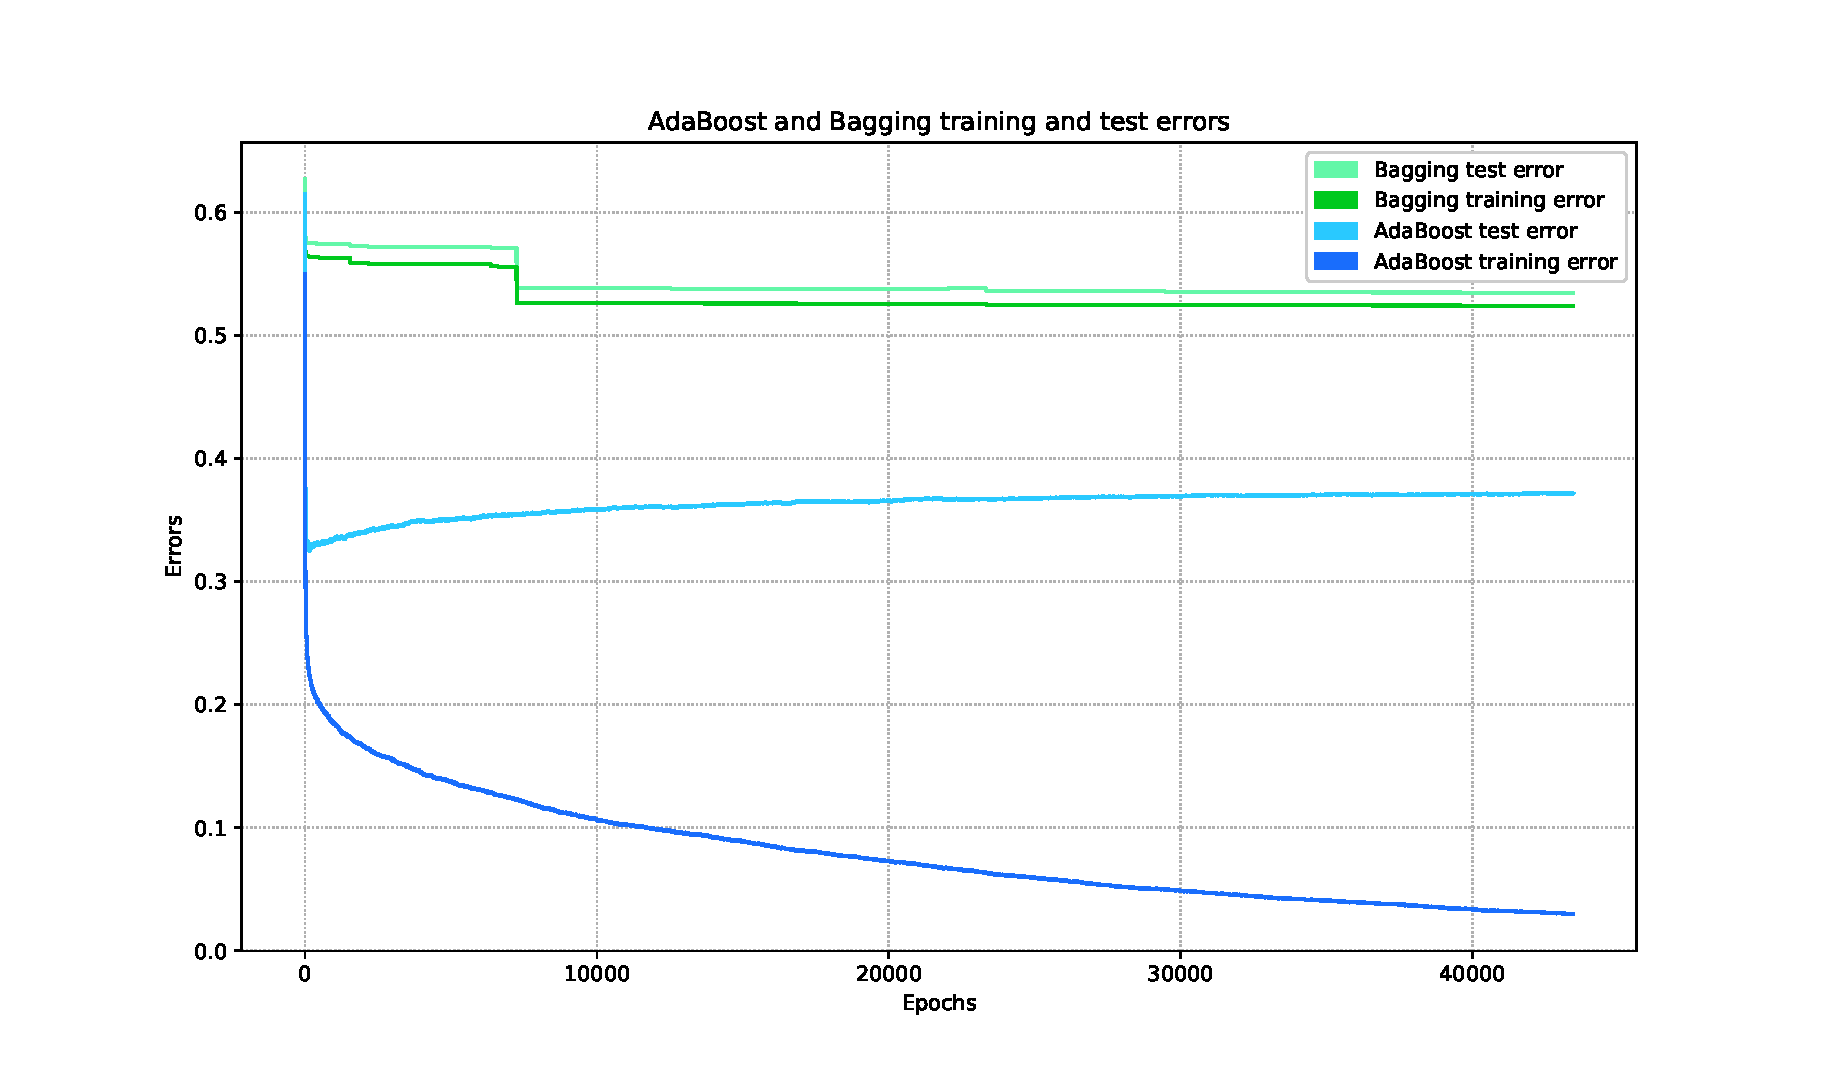
\includegraphics[width=0.5\textwidth]{figs/report_k2.eps}
	}
	\subfloat[K = 5]{
		\label{ref_k5}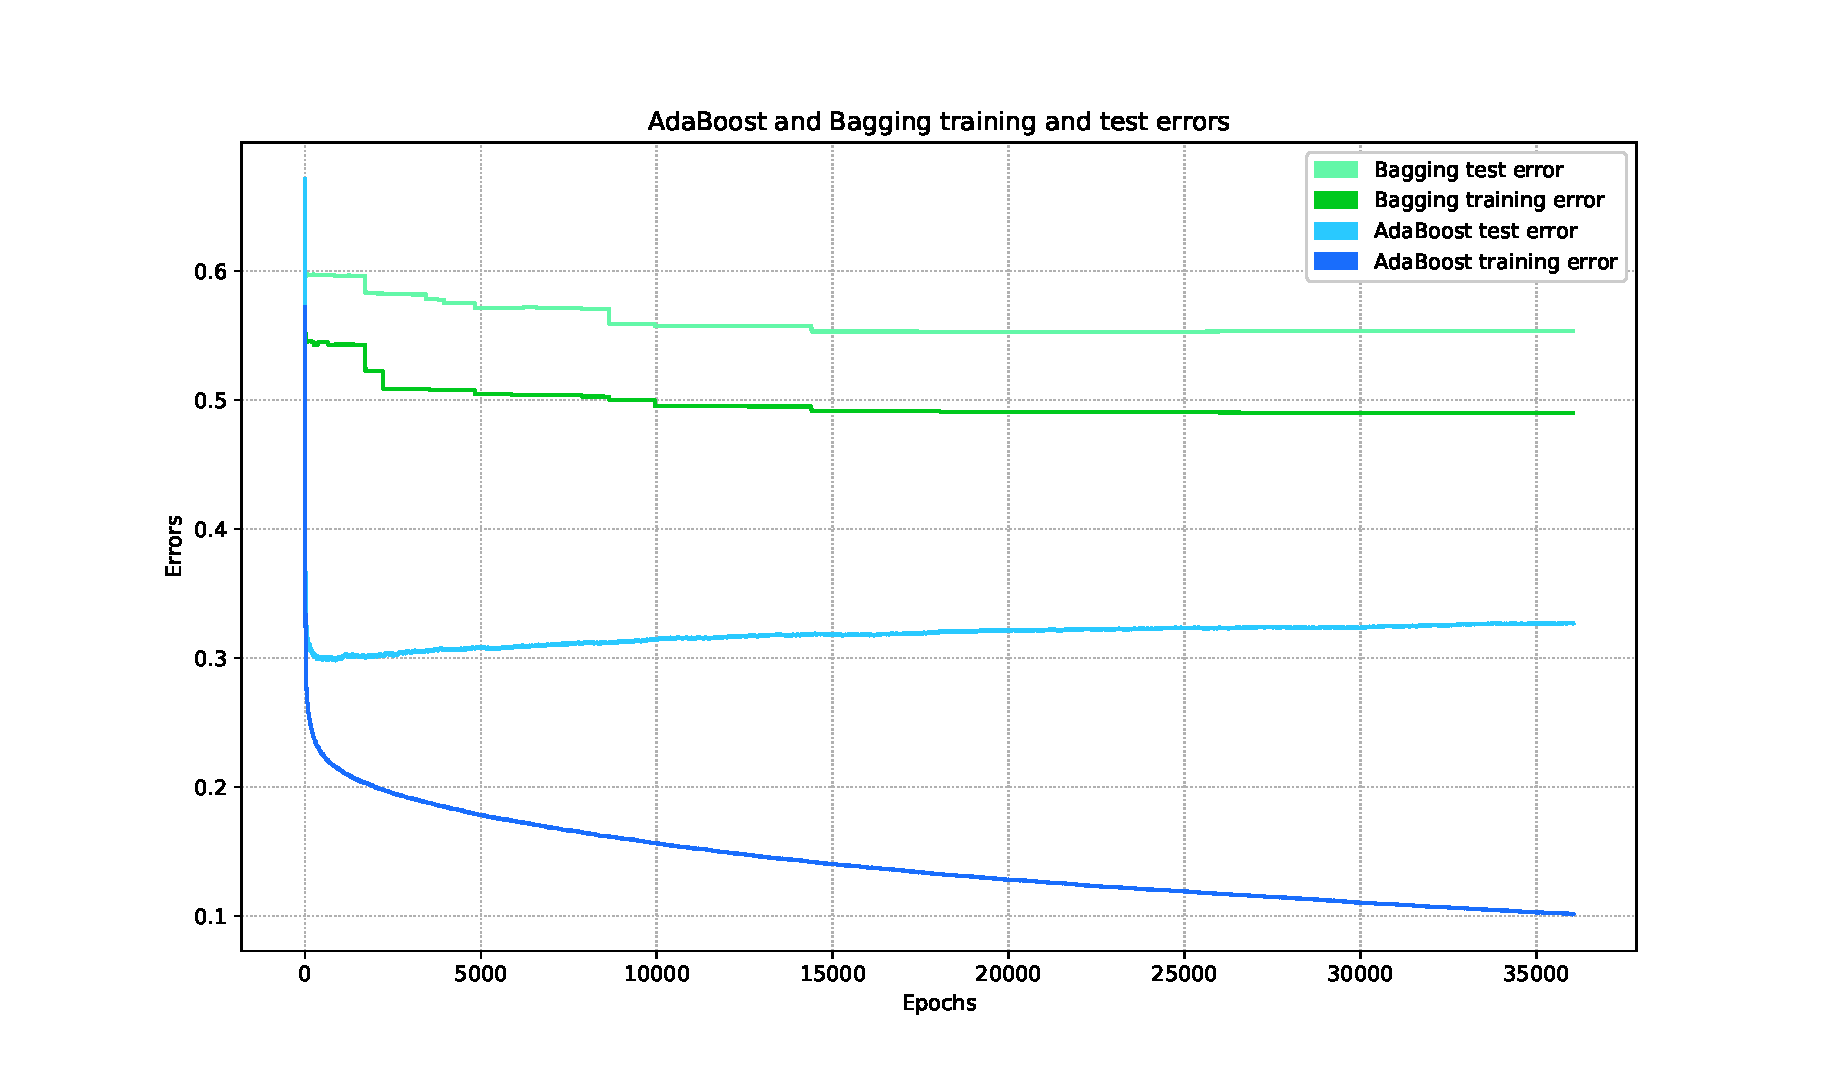
\includegraphics[width=0.5\textwidth]{figs/report_k5.eps}
	}
	\\
	\subfloat[K = 20]{
		\label{ref_k20}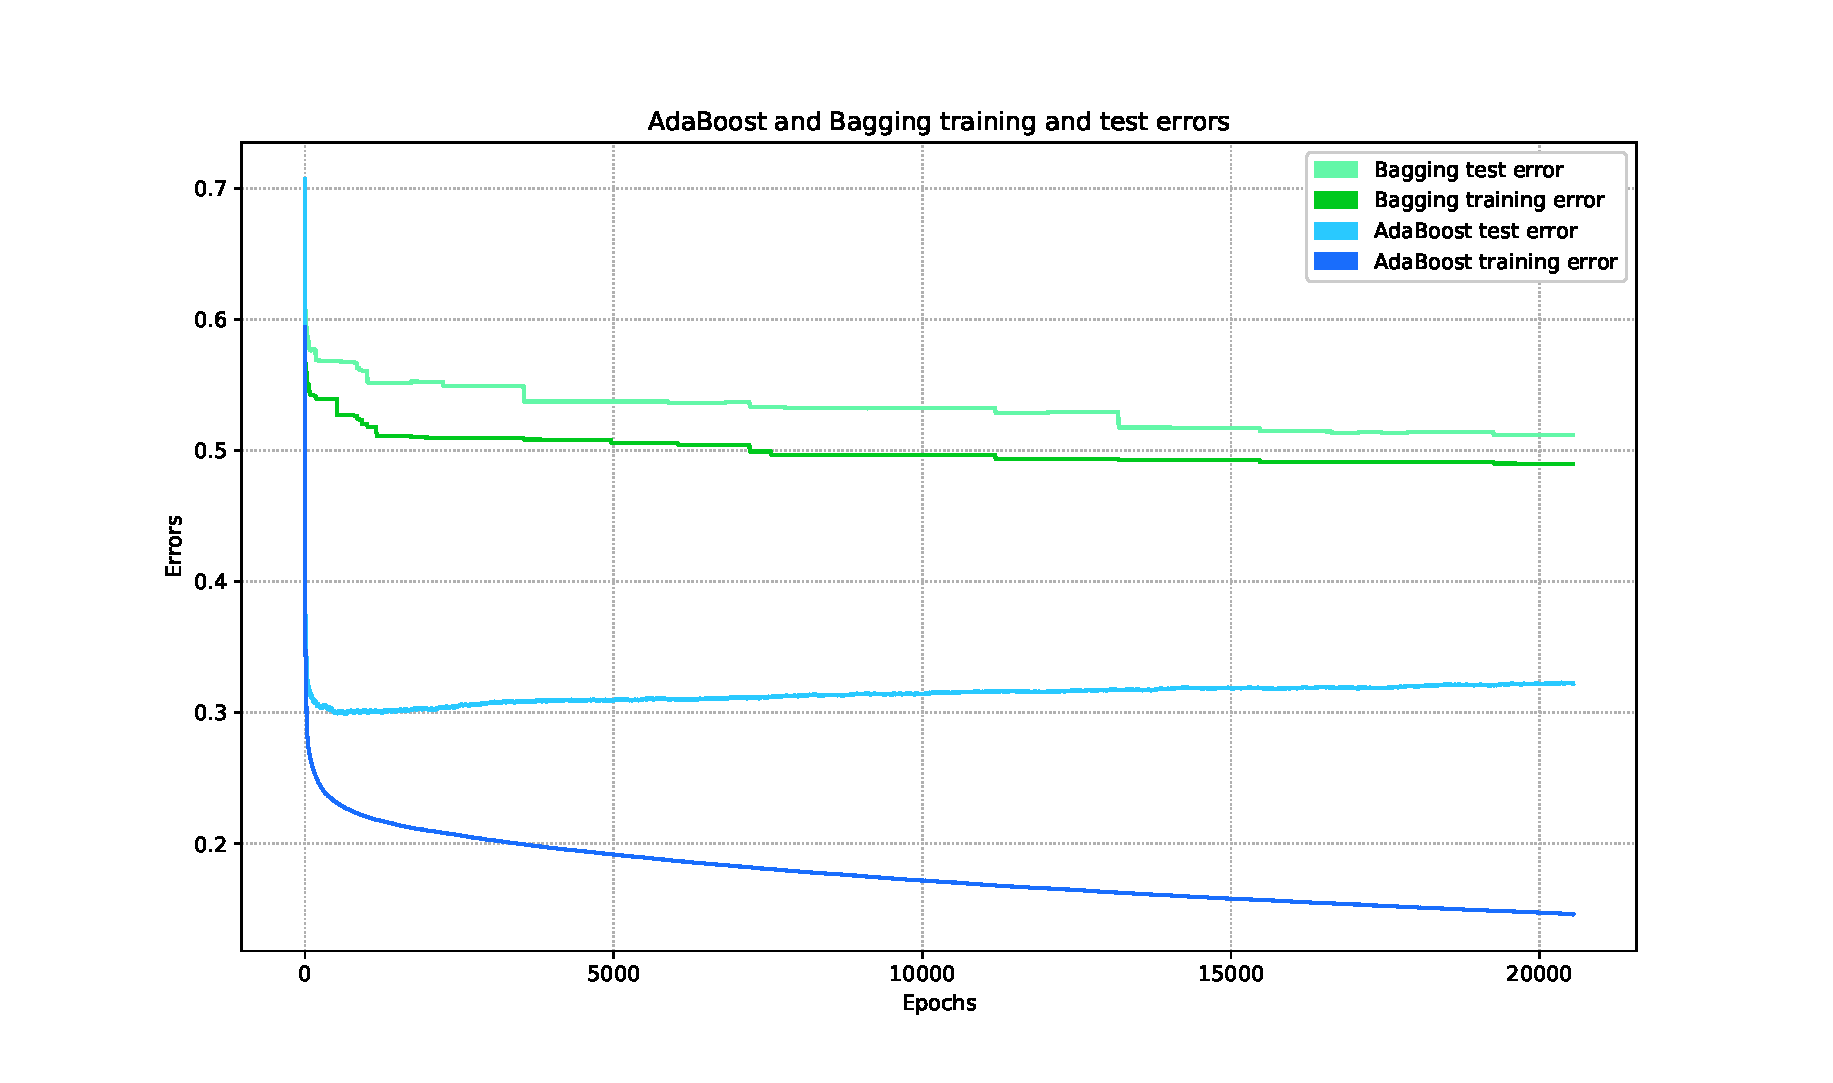
\includegraphics[width=0.5\textwidth]{figs/report_k20.eps}
	}
	\subfloat[K = 750]{
		\label{ref_k750}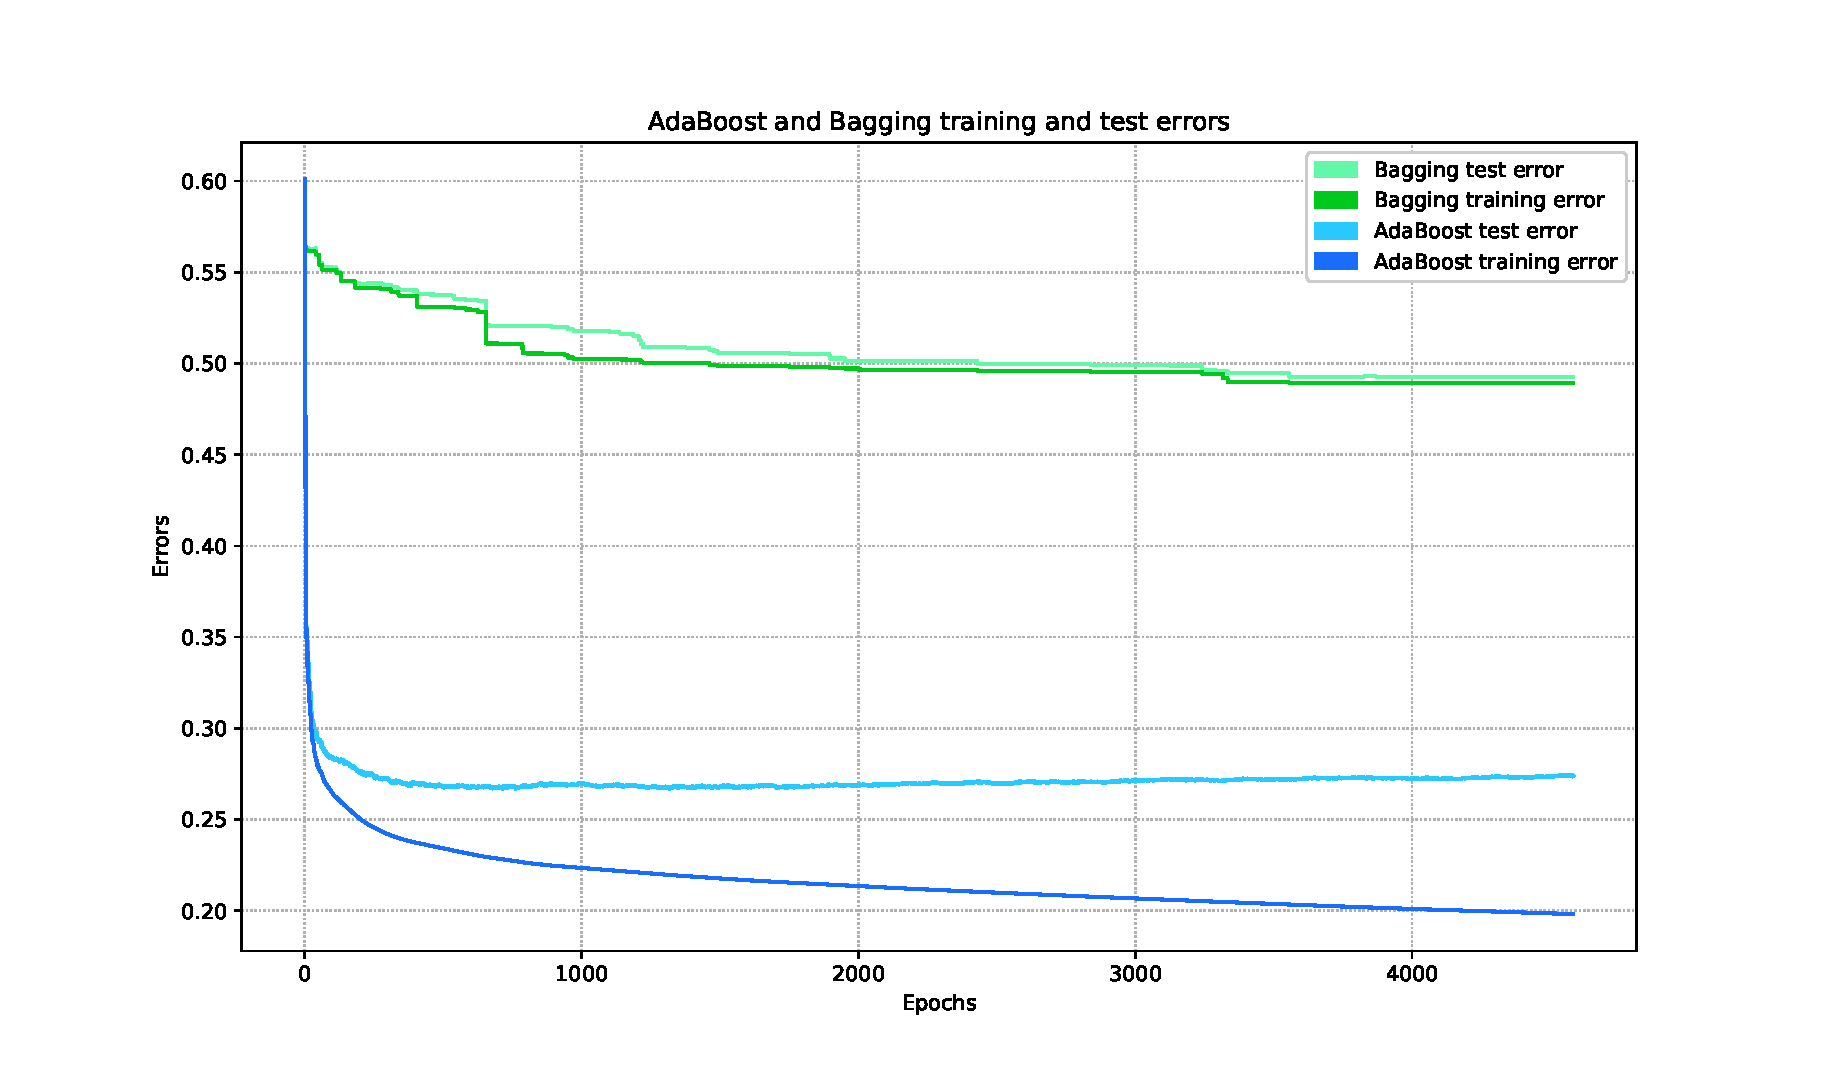
\includegraphics[width=0.5\textwidth]{figs/report_k750.eps}
	}
	\caption{\label{fig:plots_kfold}Four examples of execution over four different K-fold cross validation.}
\end{figure}
In \autoref{fig:plots_kfold}, we provide four examples of execution for both AdaBoost and Bagging reporting the training and test error over thousands of epochs with different $K$ parameters. Notice that in each of the four example provided, the AdaBoost's results suggests that the algorithm starts to overfit way before $1000$ epochs executed. On the other hand, we couldn't be able to provide the best T value for bagging algorithm with that amount of epochs.
Table \autoref{tab:results} summarize all the results for all the $K$-fold experiments on AdaBoost.

\begin{table}
\centering
\begin{tabular}{|c|c|c|}
	\hline
	K & Best T value & Test Error \\
	\hline
	2 & 144 & 0.325198412698413 \\
	\hline
	3 & 260 & 0.308068783068783 \\
	\hline
	5 & 873 & 0.298148148148148 \\
	\hline
	10 & 673 & 0.302050264550265 \\
	\hline
	20 & 650 & 0.29861 \\
	\hline
	50 & 998 & 0.291995716127904 \\
	\hline
	150 & 637 & 0.281324092409241 \\
	\hline
	300 & 563 & 0.272647058823529 \\
	\hline
	750 & 714 & 0.26634920634921 \\
	\hline
\end{tabular}
\caption{All the results varying the parameter $K$ in the cross-validation}
\label{tab:results}
\end{table}
